\section{Metodologia}

\begin{frame}{Sistema Inteligente}

    \[\boxed{\text{\alert<2>{Inteligência artificial}} + \text{Engenharia} = \text{Sistema Inteligente}}\] 
\end{frame}

\begin{frame}{Redes Neurais (Artificiais)}
\pause
\begin{figure}
\centering
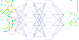
\includegraphics{figures/rede_neural.pdf}
\end{figure}
\pause
\begin{table}
\centering
\begin{tabular}{|l|l|l|}
    \hline
    Caso & \(x_i\)           & \(y_i\)             \\ \hline
    SHM  & dados PZT         & \alert<4>{problemas no trilho} \\ \hline
    VANT & \(S_0\) e \(S_i\) & forças atuantes     \\ \hline
\end{tabular}
\end{table}
\end{frame}

\begin{frame}{Implementação}
\pause
\begin{itemize}
    \item \textbf{SHM}
        \begin{itemize}
            \item<3-4> Utilização do algoritmo já disponível.
            \item<3-4> MATLAB para geração de dados.
            \item<3-4> PyTorch para modelagem da rede neural.
        \end{itemize}
    \item \textbf{VANT}
    \begin{itemize}
        \item<4> Dados fornecidos pela VALE.
        \item<4> PyTorch para modelagem da rede neural.
    \end{itemize}
\end{itemize}
    
\end{frame}